\documentclass[12pt]{beamer}
\usepackage[utf8]{inputenc}
\usepackage[T1]{fontenc}
\usepackage{lmodern}
\usetheme{Berlin}
\usepackage{graphicx}
\usepackage{hanging}

\begin{document}
	\author{Lucas Blakeslee}
	\title{Entropy in DNA}
	%\subtitle{An entropy-reduction based method}
	%\logo{}
	\institute{Institute for Computing in Research}
	\date{\today}
	%\subject{}
	%\setbeamercovered{transparent}
	%\setbeamertemplate{navigation symbols}{}
	\begin{frame}[plain]
		\maketitle
	\end{frame}
	
	\section{Introduction}
	
	\begin{frame}{Entropy}
		What is \emph{entropy}?
	\end{frame}

	\begin{frame}{Shannon Entropy}
		\begin{list}{}
			\item Claude Shannon's 1940s work on telephone lines
			\item How can one quantify the information "lost"?
		\end{list}
	\begin{equation}
		H=-K\sum _{i=1}^{n}p(i)\log p(i)
	\end{equation}
	Where H is entropy, K is a positive constant, and $p(i)$ is the probability that a system will be in state $i$.
	\end{frame}

	\begin{frame}{Shannon Entropy}
		Common modern definition:
		\begin{equation}
			H(P) = -\sum_{i=1}^n\, p_i\log_2 (p_i)
		\end{equation}
		Can be interpreted as the uncertainty; entropy can give insight into how good of a guess we have about the next piece of information
	\end{frame}

	\begin{frame}{Block Entropy}
		Shannon entropy can tell us about the frequency of a given letter in a sequence, but it can't tell us the relationships between them. For this, we need \emph{block entropies}
	\begin{equation}
		H_{n}= \sum _{i}p_{i}^{(n)}\log p_{i}^{(n)}
	\end{equation}
	
	Where $P_{i}^{(n)}$ are the probabilities of the combinations of n symbols. 
	\end{frame}

	\begin{frame}{Topological Entropy}
		A measure of entropy designed to describe topological dynamical systems
		\vfill
		One adaptation of topological entropy for sequences of finite length was described by Koslicki (2011):
		
		\emph{If $w$ is a finite sequence of length $|w|$, and n is the unique integer such that:}
		$4^{n}+n-1 \leq |w| < 4^{n-1} +(n+1) -1$
		\begin{equation}
			H_{top}(w) = \frac{\log_{4}(p_{w^{4^{n}+n -1}} (n))}{n}
		\end{equation}
		(In this case 4 is the number of letters in our alphabet \{A, C, T, G\})
	\end{frame}

	\section{Motivation}

	\begin{frame}{Entropy in Genetic Information}
		Previous computational biologists, namely Schmitt \& Herzel (1997) and Koslicki (2011) have explored applying Shannon and topological entropy respectively to genetic information, as well as crafting approximations to save computational time.
	\end{frame}

	\begin{frame}{Entropy in Genetic Information}
		Here we tried to create a method for calculating the entropy of genetic sequences based off information that's already known about members of a species' biological class.
		\vfill
		We have less \emph{surprise} (lower entropy), if we already know that certain subsequences are more likely for a class, like how it's not surprising for children's stories to start with \emph{``once upon a time...''}
		\vfill
		Entropy = Raw\_Entropy - Entropy\_Reduction
	\end{frame}

	\section{Methods}
	\begin{frame}{Classifying Sequences}
		
		Poisson Distribution: \newline
		\begin{equation}
			P(\lambda, k)={\frac {\lambda ^{k}e^{-\lambda }}{k!}}
		\end{equation}
		A probability distribution which can describe the probability of a given number of events occurring within a period.
		\vfill
		The following was derived:
		\begin{equation}
			\ell(k_{i}, ^k\lambda_{i}) = \sum k_{i}\ln ^t\lambda_{i} + c
		\end{equation}
		where $\ell$ is the log probability
	\end{frame}

	\begin{frame}{Classifying Sequences}
		\begin{equation}
			\ell(C_i, C_i\_expected\_T) = \sum C_i log(C_i\_expected\_T)  + K\newline
		\end{equation}
		\vfill
		where $C_i$ is the count of $i^{th}$ subsequence \newline
		and $T$ is the type of organism
		\vfill
		Find the organism type T which maximizes the probability
	\end{frame}

	\begin{frame}{Sequence Databases}
		Created a database of average sequences using multiple members of a class \newline
		\texttt{
		\begin{center}
			\begin{tabular}{ c c }
				\hline
				TTTTTATTTTTTAAA & 6.25 \\  
				TTTTTTTATTTTTTC & 3.75  \\
				TTTTTTTTATTTTTT & 3.375
\\
				AAAAAATATTAAAAA & 3.75
\\
				TTTTATTTTTTCTTT & 7.5
\\
				TAAAAAATAAAAAAA & 4.625
\\
				TATTTTTTTATTTTT & 3.75
\\
				\hline
			\end{tabular}
		\end{center}
	}
	\end{frame}

	\begin{frame}{}
		\begin{center}
			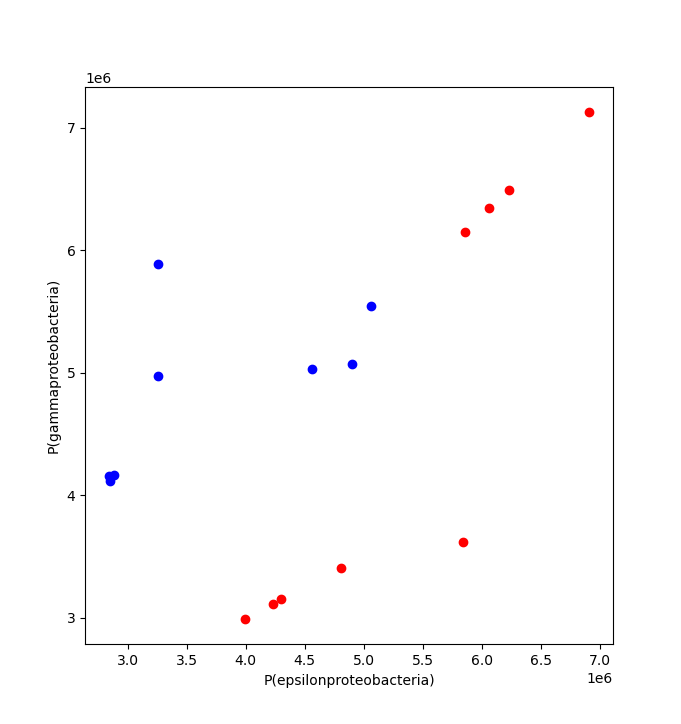
\includegraphics[scale=0.35]{find-likely-class-test.png}
		\end{center}
	\end{frame}

	\begin{frame}{Classifying Sequences}
		Subsequences might not be the best way to identify class.
		\vfill
		Repeating subsequences may well not be Poisson random.
	\end{frame}

	\section{Results}
	\begin{frame}{Classifying Sequences}
		Microsatellites are sequences that repeat thousands of times in a genome, made up of small building blocks (e.g. GCGCGCGC or ATGATGATGATG).
		\vfill
		We tried de-weighting large numbers of repeats.
	\end{frame}

	\begin{frame}{}
		To do so, we defined a function $f$ given the counts in an unknown sequence $C_{i}$, and the expected counts averaged from a class $E_{i}$. \vfill
		\begin{equation}
			f = \frac{\sum( \log(C_{i})  \log(E_{i}) )}{\sqrt{\sum(\log(C_{i})^{2})    \sum(\log(E_{i})^{2}))}}
		\end{equation}
	\end{frame}

	\begin{frame}{}
		\begin{center}
			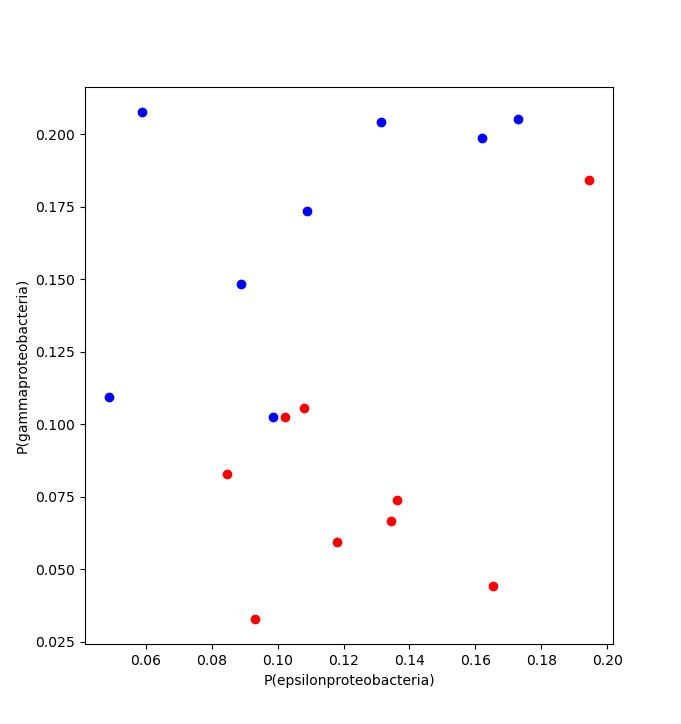
\includegraphics[scale=0.35]{func_test_2.png}
		\end{center}
	\end{frame}

	\section{Acknowledgements}
	\begin{frame}{Acknowledgements}
		I would like to thank my mentor, David Palmer, for providing invaluable help and guidance.
		\vfill
		I would also like to thank ICR and everyone involved for helping create these opportunities and this community.
	\end{frame}

	\section{References}
	\begin{frame}{References}
		\footnotesize
		\begin{hangparas}{.25in}{1}
		Koslicki, D. (2011). Topological entropy of DNA sequences. \emph{Bioinformatics}, 27(8), 1061–1067. https://doi.org/10.1093/bioinformatics/btr077 

		Schmitt, A. O., \& Herzel, H. (1997). Estimating the Entropy of DNA Sequences. \emph{Journal of Theoretical Biology}, 188(3), 369–377. https://doi.org/10.1006/jtbi.1997.0493 
		
		Shannon, C. E., \& Weaver, W. (1949). The mathematical theory of communication. \emph{Urbana: University of Illinois Press}.
		\end{hangparas}
	\end{frame}
\end{document}